% Standalone RAKL authority partial-order Hasse diagram (Paper I).
% Build:  pdflatex authority_hasse.tex  -> authority_hasse.pdf
\documentclass[border=6pt]{standalone}
\usepackage{tikz}
\usepackage{amsmath}
\usepackage{helvet}\renewcommand{\familydefault}{\sfdefault}
\usetikzlibrary{positioning,arrows.meta,fit,backgrounds,calc}
\begin{document}
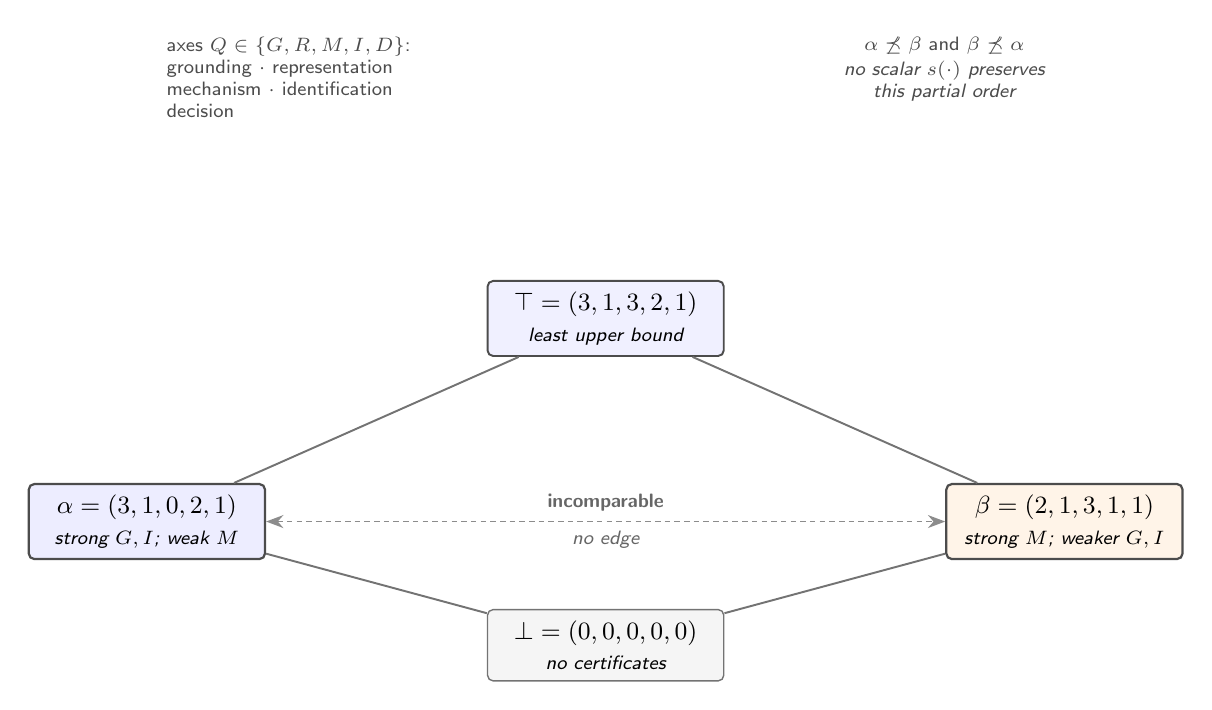
\begin{tikzpicture}[
  font=\small,
  >={Stealth[length=2.2mm]},
  vec/.style={rounded corners=2pt, draw=black!55, line width=0.5pt, align=center,
              inner sep=4pt, minimum height=9mm, minimum width=30mm, fill=white},
  inc/.style={vec, draw=black!70, line width=0.8pt},
  cover/.style={-, line width=0.7pt, draw=black!55},
  lbl/.style={font=\scriptsize\itshape, text=black!60},
  node distance=16mm and 34mm,
]
% axis legend (top-left)
\node[align=left, font=\scriptsize, text=black!70, anchor=north west]
  (axes) at (-5.7,3.7)
  {axes $Q\in\{G,R,M,I,D\}$:\\grounding $\cdot$ representation\\mechanism $\cdot$ identification\\decision};

% ---- top: join = coordinatewise max ----
\node[vec, fill=blue!6, draw=black!70, line width=0.7pt] (top)
  {$\top=(3,1,3,2,1)$\\{\scriptsize\itshape least upper bound}};

% ---- incomparable pair, side by side, NO edge between them ----
\node[inc, below left=of top, xshift=6mm, fill=blue!7]  (a)
  {$\alpha=(3,1,0,2,1)$\\{\scriptsize\itshape strong $G,I$; weak $M$}};
\node[inc, below right=of top, xshift=-6mm, fill=orange!9] (b)
  {$\beta=(2,1,3,1,1)$\\{\scriptsize\itshape strong $M$; weaker $G,I$}};

% ---- bottom ----
\node[vec, fill=black!4, below=32mm of top] (bot)
  {$\bot=(0,0,0,0,0)$\\{\scriptsize\itshape no certificates}};

% ---- cover edges of the product order (Hasse: no edge alpha--beta) ----
\draw[cover] (bot) -- (a);
\draw[cover] (bot) -- (b);
\draw[cover] (a)   -- (top);
\draw[cover] (b)   -- (top);

% ---- incomparability annotation between alpha and beta ----
\draw[<->, line width=0.5pt, draw=black!45, dash pattern=on 2pt off 1.5pt]
  (a.east) -- node[above, font=\scriptsize\bfseries, text=black!60]{incomparable}
              node[below, lbl]{no edge} (b.west);

% ---- "no scalar collapse" note ----
\node[align=center, font=\scriptsize, text=black!70, anchor=north east]
  at (5.7,3.7)
  {$\alpha\not\preceq\beta$ and $\beta\not\preceq\alpha$\\[1pt]
   {\itshape no scalar $s(\cdot)$ preserves}\\{\itshape this partial order}};
\end{tikzpicture}
\end{document}
